
%----------------------------------------------------------------------------------------
%	PACKAGES AND THEMES
%----------------------------------------------------------------------------------------

\documentclass{beamer}
\mode<presentation> {
\usetheme{Berlin}
}
\AtBeginSection[]{
  \begin{frame}
  \vfill
  \centering
  \begin{beamercolorbox}[sep=8pt,center,shadow=true,rounded=true]{title}
    \usebeamerfont{title}\insertsectionhead\par%
  \end{beamercolorbox}
  \vfill
  \end{frame}
}
\usepackage{graphicx} % Allows including images
\usepackage{booktabs} % Allows the use of \toprule, \midrule and \bottomrule in tables

%----------------------------------------------------------------------------------------
%	TITLE PAGE
%----------------------------------------------------------------------------------------
\titlegraphic{
\includegraphics[width=5.5cm]{photo/ohm_logo.png}}

\title[Department of Computer Science]{IT-based Automatic Text Summarization with the Use of Textgeneration Methods} % The short title appears at the bottom of every slide, the full title is only on the title page
\author{L\"ohr Tim} 
\institute[Prof. Dr. Alfred Holl] % Your institution as it will appear on the bottom of every slide, may be shorthand to save space
{
Technische Hochschule Nürnberg Georg Simon OHM\\ % Your institution for the title page
\medskip
\textit{Bachelor Thesis | Business Information Systems and Management} 
}
\date{\today} % Date, can be changed to a custom date
%----------------------------------------------------------------------------------------
\begin{document}

\begin{frame}
\titlepage % Print the title page as the first slide
\end{frame}
%----------------------------------------------------------------------------------------
\begin{frame}
\frametitle{Overview} % Table of contents slide, comment this block out to remove it
\tableofcontents % Throughout your presentation, if you choose to use \section{} and \subsection{} commands, these will automatically be printed on this slide as an overview of your presentation
\end{frame}
%
%----------------------------------------------------------------------------------------
%	PRESENTATION SLIDES
%----------------------------------------------------------------------------------------

%------------------------------------------------
\section{Introduction}

%------------------------------------------------

\begin{frame}
\frametitle{Clarify the Keywords}
Artificial Intelligence is increasingly finding its way more and more into businesses. 
\begin{columns}
	\column{0.3\textwidth}
	\begin{figure}
		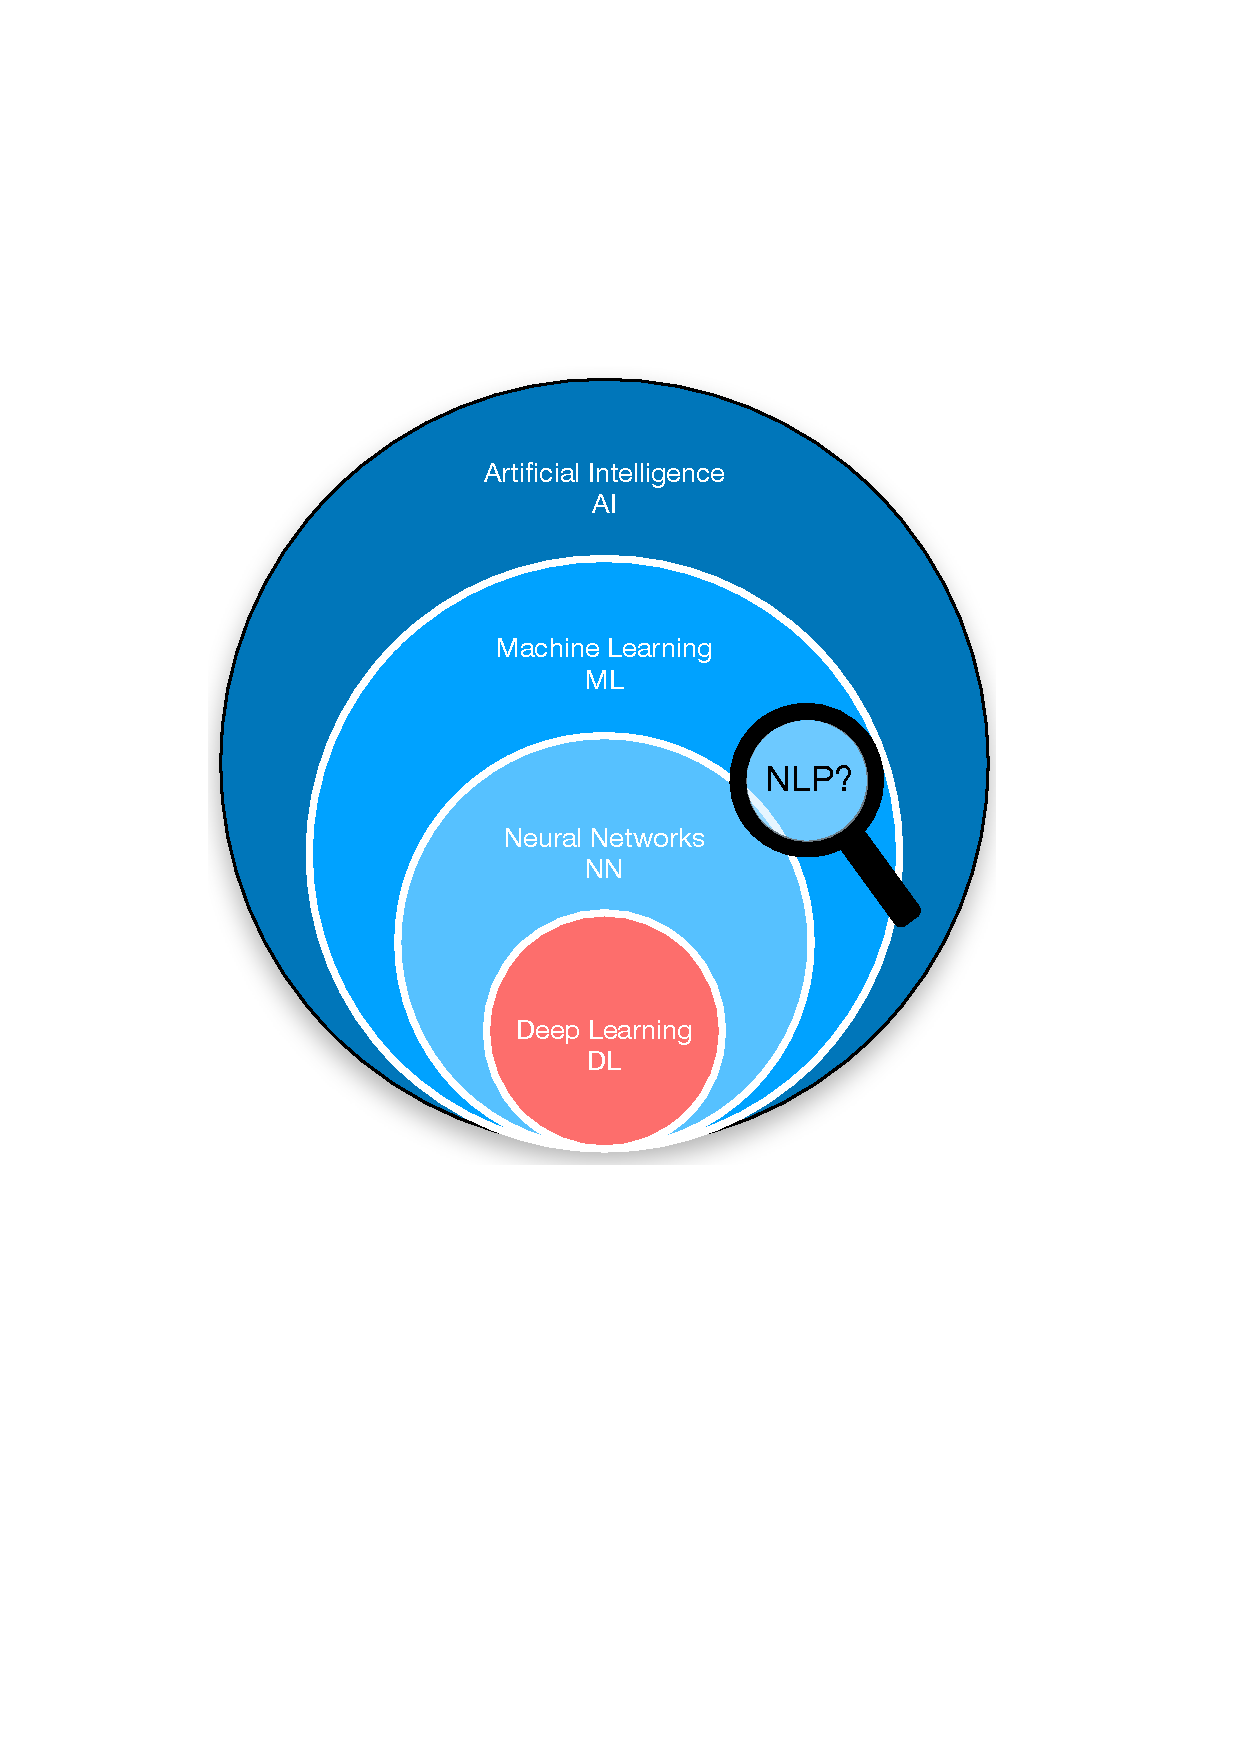
\includegraphics[width=1.15\linewidth]{photo/intro_0}
	\end{figure}
	\column{0.6\textwidth}
	\begin{block}{Famous phrases for Advertisement}
		\begin{enumerate}
			\item \textit{Our product is powered now by AI!} 
			\item \textit{We now use Deep Learning for a better performance!}
		\end{enumerate}
	\end{block}
\textbf{In conclusion:} Deep Learning is a technique making use of Neural networks. Those are methods of Machine Learning, which 
 itself is just an application of the entire AI ecosystem.
\end{columns}
\end{frame}

%------------------------------------------------

\begin{frame}
\frametitle{Localize my thesis within this Ecosystem}
\begin{block}{NLP}
	Natural Language Processing (NLP) deals with language and manipulates it to gain new information from it or perform other related tasks such as Text Summarization.
\end{block}

\begin{center}
	\textbf{What do I use?} \\
\end{center}

Using Natural Language Processing (NLP) with e.g. Hidden Markov Models is categorized as Machine Learning, whereas using Sequence Networks with e.g. the Tensorflow library is categorized Deep Learning. That is what my prototype uses.

\end{frame}

%------------------------------------------------
\section{State of the Art}
%---------------------------------------------
\begin{frame}
\frametitle{Text Generation}
Isn't my topic about Text Summarization? What is Text Generation?
\begin{figure}
	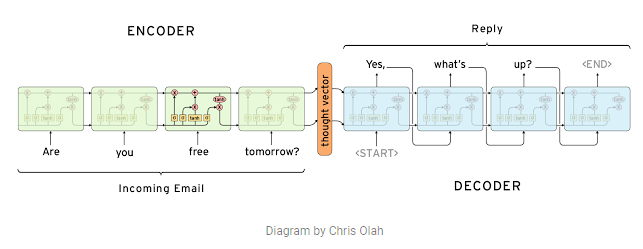
\includegraphics[width=0.9\linewidth]{photo/encoder_decoder}
\end{figure}
This is Text Generation performed by eight LSTM cells, which are split into four encoder and four decoder cells.
\end{frame}
%
%------------------------------------------------
%
\begin{frame}
\frametitle{Text Generation: commonly used technologies}
\begin{columns}[c] % The "c" option specifies centered vertical alignment while the "t" option is used for top vertical alignment

\column{.45\textwidth} % Left column and width
\textbf{State of the Art in ascending order}
\begin{enumerate}
\item Recurrent Neural Networks (RNN)
\item Long Short Term Memory (LSTM)
\item Sequence to Sequence Models
\item Encoder Decoder
\item Attention based Models
\end{enumerate}

\column{.5\textwidth} % Right column and width

\begin{block}{Definition Text Generation}
Text Generation is a generic term for the output part of an automatic text summarizer (decoder part from the last slide). In order to understand Text Summarization, we need to know about Text Generation.
\end{block}
\end{columns}
\end{frame}

%------------------------------------------------

\begin{frame}
\frametitle{Text Summarization}
To make this clear. Text Generation is the tool which produces output language, based on the preprocessed input language. Text Summarization focusses on making use of this techniques, for generating fewer words out of the original input sentence with the preferably same information content. \\
\textit{This is commonly known as summarization.}

\begin{block}{Today}
	Text Summarization in 2020 is almost not distinguishable anymore from a human summarization. A famous example is that Google uses it to automatically generate headlines for their news section, which is basically an summarization or abstraction from the news itself.
\end{block}
\end{frame}

%------------------------------------------------

\begin{frame}
	\frametitle{Latest Technologies in Text Summarization}
	\begin{columns}[c]
		
		\column{.5\textwidth} % Right column and width
		\begin{block}{Deep Learning}
			
			Deep Learning is the best technique for Text Summarization in 2020. E.g. the famous technology \textit{Attention,} which is based on the LSTM Neural Network, was published and open sourced by Google. Other technologies just build further up on this concept.
		\end{block}
	
	   \column{.5\textwidth} % Right column and width
	   \textbf{State of the Art in ascending order}
		\begin{enumerate}
			\item Extractive approaches
			\item Abstractive approaches
			\item Attention 
			\item Pointer Generator Networks
			\item Transfer Learning
		\end{enumerate}
	\end{columns}

\end{frame}

%------------------------------------------------

\begin{frame}
	\frametitle{How does the machine understand our language?}
	\begin{columns}
		\column{.7\textwidth} % Right column and width
		\begin{figure}
			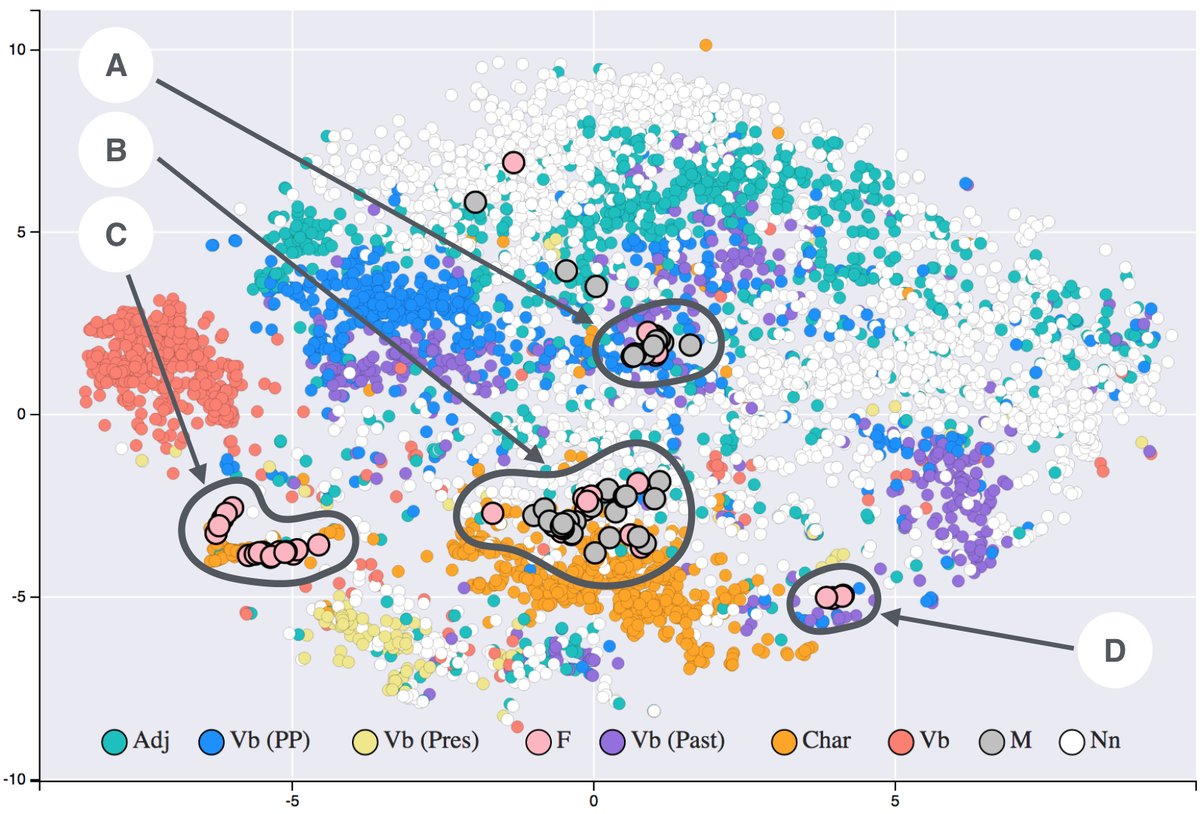
\includegraphics[width=.9\linewidth]{photo/generate_text}
		\end{figure}
	   Here are shown the distribution of words by their word types in the vector space.
	
				\column{.3\textwidth} % Right column and width
				Well it acutally doesn't. The machine learns the structure of sentences and occurences of words in our language. In order to make them computable for the algorithm, the words will be vectorized.
	\end{columns}
	
\end{frame}

%------------------------------------------------

\section{Prototype}
%--------------------------------------------

\begin{frame}
\frametitle{Basic structure}
\begin{figure}
	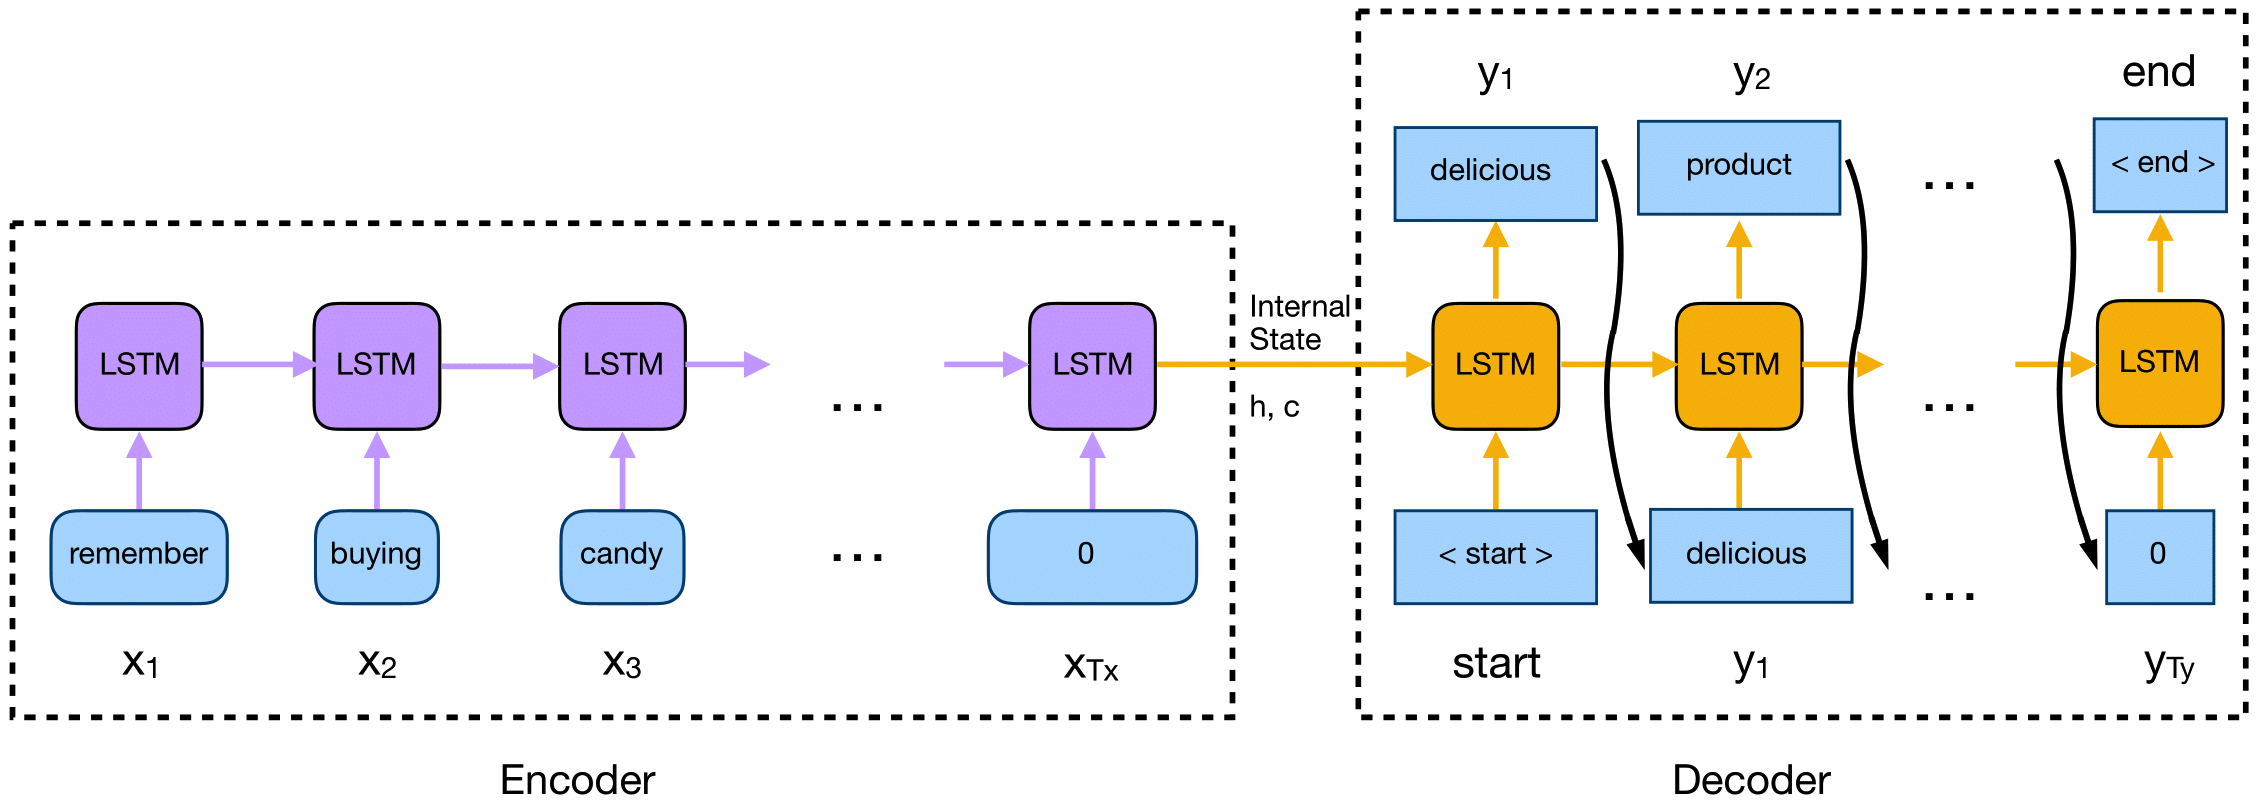
\includegraphics[width=.9\linewidth]{photo/infer-1}
\end{figure}

\begin{block}{Architecture}
	My prototype is built upon multiple LSTM cells which were extended by the Attention Layer from Google. It took around ~3.5 hours to train on my PC with around 222.000 training data points.
\end{block}
\end{frame}

%------------------------------------------------
\begin{frame}
\frametitle{Model results}
\begin{figure}
	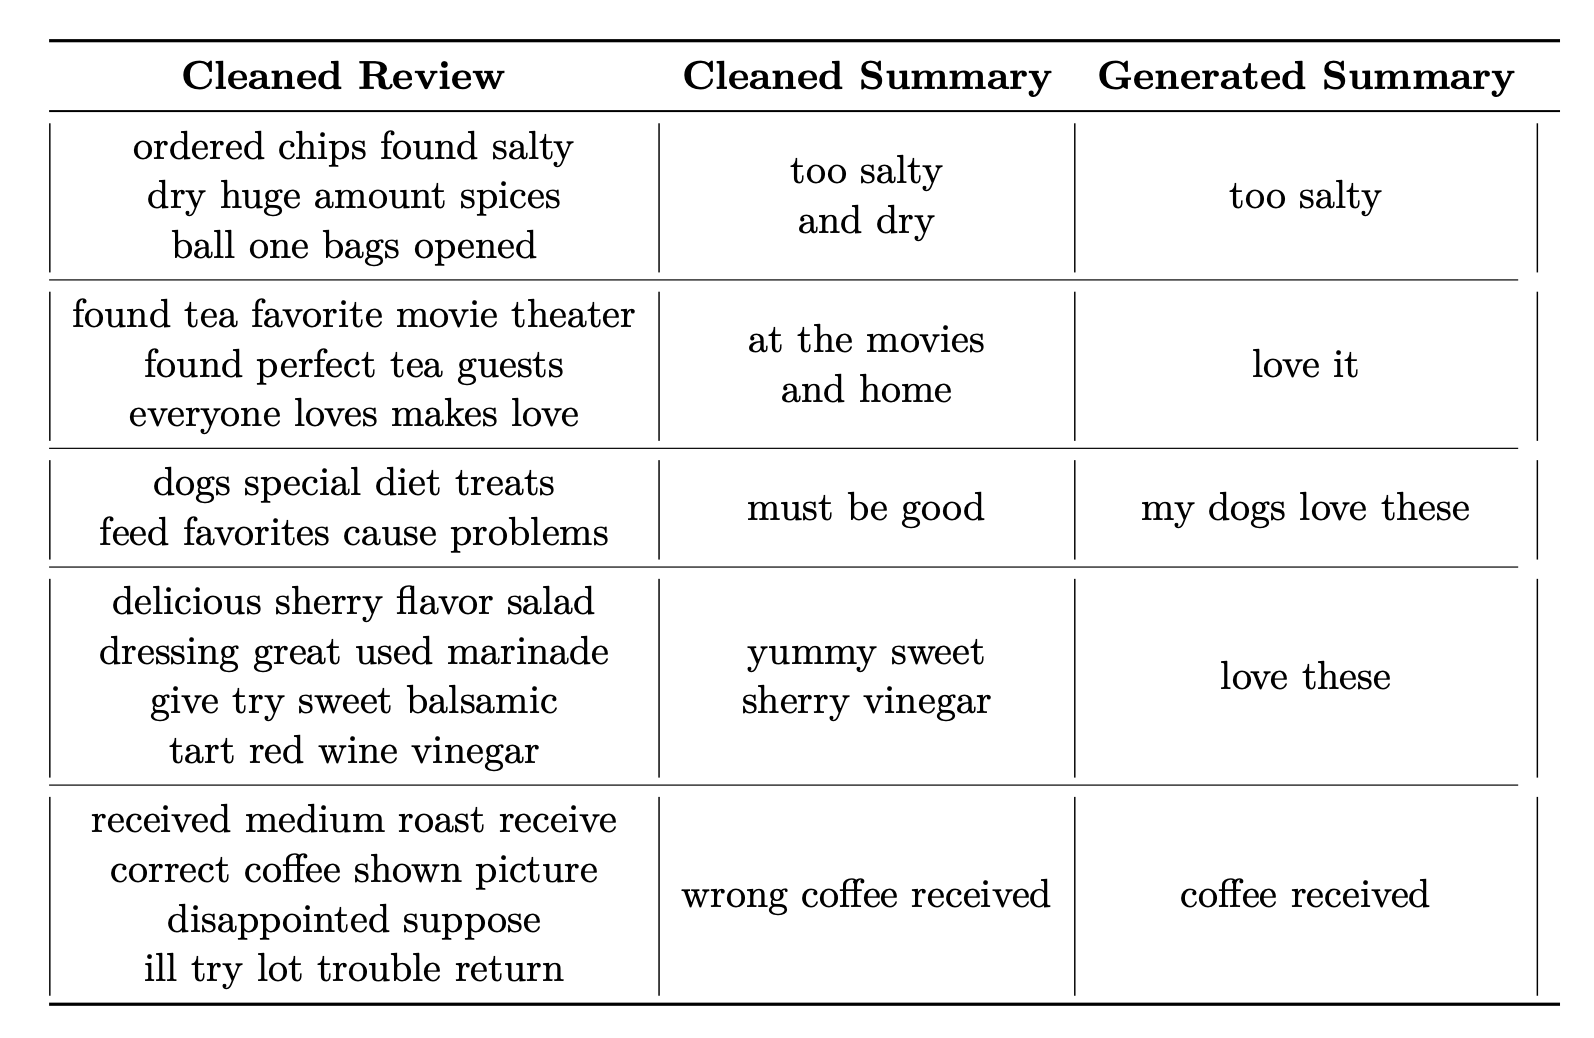
\includegraphics[width=0.9\linewidth]{photo/prototype_outputs}
\end{figure}
\end{frame}

%------------------------------------------------
\section{Evaluation}
%--------------------------------------------
\begin{frame}
	\frametitle{Evaluate the summary}
It was necessary to clean the input text before funneling it into the model. The \textbf{cleaned summary} is the ground truth which was provided together with the dataset as labels. It can be seen, that the most important words were captures and only minor mistakes occured.

\begin{figure}
	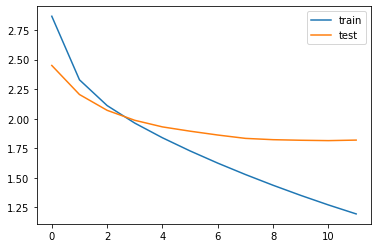
\includegraphics[width=0.5\linewidth]{photo/eval}
\end{figure}

This is the Loss curve for my model from the Neural Network.
\end{frame}

%------------------------------------------------

\end{document} 